\documentclass[crop,tikz,convert={outext=.svg,command=\unexpanded{pdf2svg \infile\space\outfile}},multi=false]{standalone}

\usepackage{ifthen}
\usetikzlibrary{arrows}
\usetikzlibrary{positioning}
\usetikzlibrary{shapes}
\usetikzlibrary{calc}

\tikzstyle{state}=[circle, fill=gray!20, minimum width = 2cm]
\tikzstyle{alice}=[circle, fill=red!20, minimum width = 1cm]
\tikzstyle{bob}=[circle, fill=blue!20, minimum width = 1cm]
\tikzstyle{client}=[circle, fill=gray!20, minimum width = 1cm]
\tikzstyle{buf}=[rectangle, draw, minimum width = 1cm, minimum height = 1cm]

\begin{document}
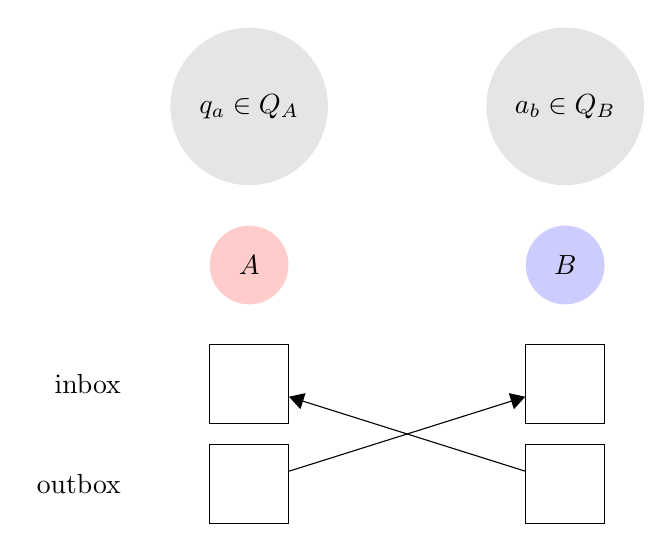
\begin{tikzpicture}[>=triangle 60]
    % nodes
    \node[alice] (A) {$A$};
    \node[bob, right=3cm of A] (B) {$B$};
    \node[state, above=0.5cm of A] (AQ) {$q_a \in Q_A$};
    \node[state, above=0.5cm of B] (BQ) {$a_b \in Q_B$};

    \node[buf, below=0.5cm of A] (Ain) {};
    \node[buf, below=0.25cm of Ain] (Aout) {};
    \node[buf, below=0.5cm of B] (Bin) {};
    \node[buf, below=0.25cm of Bin] (Bout) {};

    \node[left=of Ain] () {inbox};
    \node[left=of Aout] () {outbox};

    \draw[->] (Aout) -- (Bin);
    \draw[->] (Bout) -- (Ain);
\end{tikzpicture}
\end{document}
